\chapter{Counting Techniques}

When outcomes are equally likely, $P(A) = |A|/|S|$, so we need systematic ways to count
large sets without listing them. This chapter collects the standard tools.

\section{The addition and multiplication rules}

\begin{theorem}[Addition rule]
If a job can be done in one of two mutually exclusive ways, the first in $p$ ways and the
second in $q$ ways, then the job can be done in $p+q$ ways. (In set language:
$|A\cup B| = |A|+|B|$ for disjoint $A$, $B$.)
\end{theorem}

\begin{theorem}[Multiplication rule]
If a job consists of two stages, the first of which can be done in $p$ ways and, for each
of those, the second can be done in $q$ ways, then the job can be done in $pq$ ways. More
generally a $k$-stage job with $n_1, n_2, \dots, n_k$ choices at the successive stages can
be done in $n_1 n_2\cdots n_k$ ways.
\end{theorem}

The word ``and'' typically signals multiplication and ``or'' (for disjoint cases) addition.
The important point in the multiplication rule is that the \emph{number} of choices at
each stage must not depend on the earlier choices, even if the choices themselves do.

\begin{example}[Licence plates]
An Ontario-style plate has $4$ letters followed by $3$ digits. There are
$26^4 \cdot 10^3 = 456\,976\,000$ possible plates. If letters may not repeat, there are
$26\cdot 25\cdot 24\cdot 23 \cdot 10^3 = 358\,800\,000$.
\end{example}

\begin{example}[Two dice, revisited]
The number of ordered outcomes of two dice is $6\times 6 = 36$; the number with
different faces is $6\times 5 = 30$, so $P(\text{different faces}) = 30/36 = 5/6$.
\end{example}


A tree diagram makes the multiplication rule concrete: with $p=3$ choices at the first
stage and $q=2$ at the second, every first-stage branch splits into the same number of
second-stage branches, giving $3\times2 = 6$ leaves.

\begin{center}
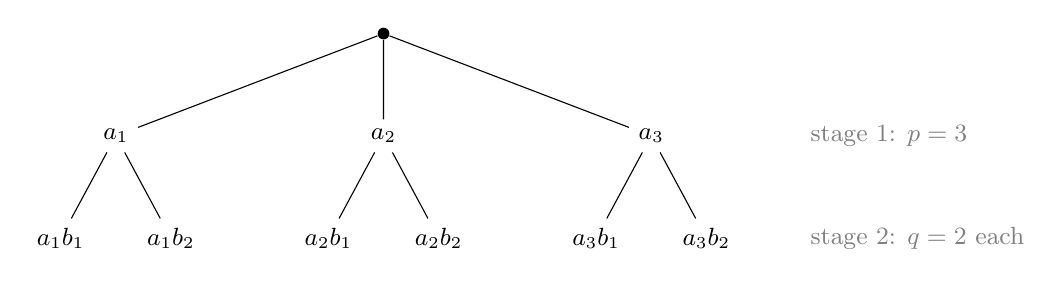
\begin{tikzpicture}[every node/.style={font=\small},
    level 1/.style={sibling distance=3.4cm, level distance=1.3cm},
    level 2/.style={sibling distance=1.4cm, level distance=1.3cm}]
  \node[circle, fill=black, inner sep=1.5pt] {}
    child { node {$a_1$} child { node {$a_1b_1$} } child { node {$a_1b_2$} } }
    child { node {$a_2$} child { node {$a_2b_1$} } child { node {$a_2b_2$} } }
    child { node {$a_3$} child { node {$a_3b_1$} } child { node {$a_3b_2$} } };
  \node[anchor=west, gray] at (5.3,-1.3) {stage 1: $p = 3$};
  \node[anchor=west, gray] at (5.3,-2.6) {stage 2: $q = 2$ each};
\end{tikzpicture}
\end{center}

\section{Permutations}

\begin{definition}[Factorial and falling factorial]
For a non-negative integer $n$, $n! = n(n-1)\cdots 2\cdot 1$ with $0! = 1$. For
$0\le k\le n$, the \emph{falling factorial} (``$n$ to $k$ factors'') is
\[
  n^{(k)} = n(n-1)(n-2)\cdots(n-k+1) = \frac{n!}{(n-k)!}.
\]
\end{definition}

\begin{theorem}[Permutations]
\begin{enumerate}
  \item The number of ways to arrange $n$ distinct objects in a row is $n!$.
  \item The number of ways to choose and arrange $k$ of $n$ distinct objects (an ordered
        selection \emph{without} replacement) is $n^{(k)}$.
  \item The number of ordered selections of $k$ objects from $n$ \emph{with} replacement
        is $n^k$.
\end{enumerate}
\end{theorem}

\begin{proof}
Multiplication rule: there are $n$ choices for the first position, $n-1$ for the second
(any object not already used), and so on, giving $n(n-1)\cdots(n-k+1)$. With replacement
there are $n$ choices at every stage.
\end{proof}

\begin{example}[Officers]
A club of $10$ people elects a president, vice-president and treasurer (different
people). The number of outcomes is $10^{(3)} = 10\cdot 9\cdot 8 = 720$.
\end{example}

\begin{example}[Random passwords]
A password consists of $6$ lowercase letters chosen uniformly at random with replacement.
The probability that no letter is repeated is
\[
  \frac{26^{(6)}}{26^6} = \frac{165\,765\,600}{308\,915\,776} \approx 0.5366.
\]
\end{example}

\subsection{The birthday problem}

\begin{example}[Birthday problem]
In a room of $n$ people, what is the probability that at least two share a birthday?
Assume $365$ equally likely birthdays (ignore Feb 29 and seasonal effects). The sample
space of birthday lists has $365^n$ equally likely outcomes, and the number of lists with
all birthdays different is $365^{(n)}$. By the complement rule,
\[
  P(\text{some shared birthday}) = 1 - \frac{365^{(n)}}{365^n}
  = 1 - \frac{365}{365}\cdot\frac{364}{365}\cdots\frac{365-n+1}{365}.
\]
For $n=23$ this is $\approx 0.5073$, and for $n=30$ it is $\approx 0.7063$. The
surprisingly small $n$ needed is because there are $\binom{n}{2}$ pairs of people, each of
which could match ($\binom{23}{2} = 253$).
\end{example}

\begin{center}
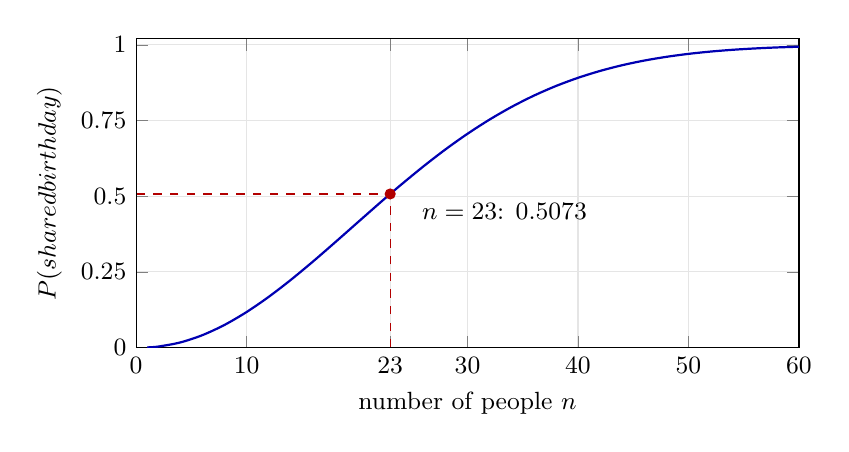
\begin{tikzpicture}
\begin{axis}[width=10cm, height=5.5cm, xmin=0, xmax=60, ymin=0, ymax=1.02,
    xlabel={number of people $n$}, ylabel={$P(\text{shared birthday})$},
    xtick={0,10,23,30,40,50,60}, ytick={0,0.25,0.5,0.75,1},
    grid=major, grid style={gray!20}, tick label style={font=\small},
    label style={font=\small}]
  \addplot[thick, blue!70!black, smooth] coordinates {(1,0) (2,0.0027) (4,0.0164) (6,0.0405) (8,0.0743) (10,0.1169) (12,0.167) (14,0.2231) (16,0.2836) (18,0.3469) (20,0.4114) (22,0.4757) (23,0.5073) (24,0.5383) (26,0.5982) (28,0.6545) (30,0.7063) (32,0.7533) (34,0.7953) (36,0.8322) (38,0.8641) (40,0.8912) (42,0.914) (44,0.9329) (46,0.9483) (48,0.9606) (50,0.9704) (52,0.978) (54,0.9839) (56,0.9883) (58,0.9917) (60,0.9941)};
  \draw[dashed, red!70!black] (axis cs:23,0) -- (axis cs:23,0.5073) -- (axis cs:0,0.5073);
  \addplot[only marks, mark=*, mark size=1.8pt, red!70!black] coordinates {(23,0.5073)};
  \node[anchor=west, font=\small] at (axis cs:25,0.45) {$n = 23$: $0.5073$};
\end{axis}
\end{tikzpicture}
\end{center}
The probability passes $1/2$ at $n=23$ and is already above $0.97$ at $n = 50$.

\section{Combinations}

\begin{definition}[Binomial coefficient]
For integers $0 \le k \le n$,
\[
  \binom{n}{k} = \frac{n^{(k)}}{k!} = \frac{n!}{k!\,(n-k)!}
\]
(read ``$n$ choose $k$''). We set $\binom nk = 0$ if $k<0$ or $k>n$.
\end{definition}

\begin{theorem}
The number of subsets of size $k$ of a set of $n$ distinct objects (an \emph{unordered}
selection without replacement) is $\binom nk$.
\end{theorem}

\begin{proof}
Count ordered selections of $k$ objects in two ways. Directly there are $n^{(k)}$. On the
other hand, each one is obtained by first choosing a subset (in $C$ ways, say) and then
ordering it (in $k!$ ways). So $n^{(k)} = C\cdot k!$.
\end{proof}

\begin{theorem}[Properties of binomial coefficients]
\begin{enumerate}
  \item $\binom nk = \binom{n}{n-k}$ (choosing who is in = choosing who is out).
  \item $\binom nk = \binom{n-1}{k-1} + \binom{n-1}{k}$ (Pascal's identity).
  \item (Binomial theorem) $(a+b)^n = \sum_{k=0}^n \binom nk a^k b^{n-k}$; in
        particular $\sum_k \binom nk = 2^n$.
  \item (Vandermonde) $\sum_{k} \binom{a}{k}\binom{b}{n-k} = \binom{a+b}{n}$.
\end{enumerate}
\end{theorem}


Pascal's identity is the rule that builds Pascal's triangle: each entry is the sum of the
two entries above it (row $n$ lists $\binom n0,\dots,\binom nn$).

\begin{center}
\begin{tikzpicture}[x=0.75cm, y=0.62cm, every node/.style={font=\small}]
  \node at (0,0) {1};
  \node[gray, anchor=east] at (-3.6,0) {$n=0$};
  \node at (-0.5,-1) {1};
  \node at (0.5,-1) {1};
  \node[gray, anchor=east] at (-3.6,-1) {$n=1$};
  \node at (-1,-2) {1};
  \node at (0,-2) {2};
  \node at (1,-2) {1};
  \node[gray, anchor=east] at (-3.6,-2) {$n=2$};
  \node at (-1.5,-3) {1};
  \node at (-0.5,-3) {3};
  \node at (0.5,-3) {3};
  \node at (1.5,-3) {1};
  \node[gray, anchor=east] at (-3.6,-3) {$n=3$};
  \node at (-2,-4) {1};
  \node[fill=orange!30, circle, inner sep=1.5pt] at (-1,-4) {4};
  \node[fill=orange!30, circle, inner sep=1.5pt] at (0,-4) {6};
  \node at (1,-4) {4};
  \node at (2,-4) {1};
  \node[gray, anchor=east] at (-3.6,-4) {$n=4$};
  \node at (-2.5,-5) {1};
  \node at (-1.5,-5) {5};
  \node[fill=blue!20, circle, inner sep=1.5pt] at (-0.5,-5) {10};
  \node at (0.5,-5) {10};
  \node at (1.5,-5) {5};
  \node at (2.5,-5) {1};
  \node[gray, anchor=east] at (-3.6,-5) {$n=5$};
  \node at (-3,-6) {1};
  \node at (-2,-6) {6};
  \node at (-1,-6) {15};
  \node at (0,-6) {20};
  \node at (1,-6) {15};
  \node at (2,-6) {6};
  \node at (3,-6) {1};
  \node[gray, anchor=east] at (-3.6,-6) {$n=6$};
  \node[anchor=west, font=\scriptsize] at (3.6,-5) {$\binom52 = \binom41 + \binom42 = 4 + 6$};
\end{tikzpicture}
\end{center}

\begin{proof}[Proof of (4)]
Choose $n$ people from a group of $a$ women and $b$ men. Splitting according to the number
$k$ of women chosen gives the left side; the right side counts the same thing directly.
\end{proof}

Vandermonde's identity is exactly the statement that the hypergeometric probabilities
(Chapter 5) sum to $1$.

\begin{example}[Committees]
A committee of $5$ is chosen at random from $6$ men and $4$ women. Find the probability
that it contains at least $2$ women.

There are $\binom{10}{5} = 252$ equally likely committees. The number with exactly $k$
women is $\binom 4k\binom{6}{5-k}$. Hence the number with at least $2$ women is
\[
  \binom42\binom63 + \binom43\binom62 + \binom44\binom61 = 6\cdot 20 + 4\cdot 15 + 1\cdot 6
  = 186,
\]
and the probability is $186/252 = 31/42 \approx 0.7381$.

Check via the complement: $0$ women gives $\binom65 = 6$ committees and $1$ woman gives
$4\cdot\binom64 = 60$, so $252 - 66 = 186$.
\end{example}

\begin{important}[Pitfall: double counting]
A tempting wrong answer to ``at least $2$ women'' is $\binom42\binom83$: choose $2$ women
first, then any $3$ of the remaining $8$ people. This counts a committee with $3$ women
several times (once for each way of designating ``the first two''), giving
$6\cdot 56 = 336 > 252$. When a count exceeds the total, you have double counted.
\end{important}

\begin{example}[Lotto 6/49]
Six numbers are drawn from $\{1,\dots,49\}$. There are $\binom{49}{6} = 13\,983\,816$
possible draws. If you hold one ticket (6 numbers), the probability of matching exactly
$3$ is
\[
  \frac{\binom63\binom{43}{3}}{\binom{49}6} = \frac{20 \cdot 12\,341}{13\,983\,816}
  = \frac{246\,820}{13\,983\,816} \approx 0.01765.
\]
\end{example}

\subsection{Card hands}

A $5$-card poker hand is an unordered selection of $5$ cards from $52$; there are
$\binom{52}{5} = 2\,598\,960$ equally likely hands.

\begin{example}[Full house]
A full house is three cards of one rank and two of another. Choose the rank of the triple
($13$ ways), which $3$ of its $4$ suits ($\binom43 = 4$), the rank of the pair (from the
remaining $12$), and its suits ($\binom42 = 6$):
\[
  P(\text{full house}) = \frac{13\cdot 4 \cdot 12 \cdot 6}{2\,598\,960} =
  \frac{3744}{2\,598\,960} \approx 0.00144.
\]
Note the ranks are chosen as $13\cdot 12$ (ordered) and not $\binom{13}{2}$, because the
two ranks play different roles (triple versus pair).
\end{example}

\begin{example}[Two pair]
Here the two paired ranks play the \emph{same} role, so they are chosen as
$\binom{13}{2} = 78$; each pair's suits in $\binom42 = 6$ ways; and the fifth card is any
of the $44$ cards not of those two ranks:
\[
  P(\text{two pair}) = \frac{78\cdot 6\cdot 6\cdot 44}{2\,598\,960} =
  \frac{123\,552}{2\,598\,960} \approx 0.0475.
\]
\end{example}

\begin{example}[Bridge hand]
In a $13$-card hand from a full deck, the probability of exactly $5$ spades is
$\binom{13}{5}\binom{39}{8}/\binom{52}{13} \approx 0.1247$.
\end{example}

\section{Arrangements when some objects are alike}

\begin{theorem}[Multinomial coefficient]
The number of distinct arrangements of $n$ objects in a row, where there are $n_1$ alike
of type $1$, $n_2$ alike of type $2$, \dots, $n_k$ alike of type $k$
($n_1+\dots+n_k = n$), is
\[
  \binom{n}{n_1, n_2, \dots, n_k} = \frac{n!}{n_1!\, n_2! \cdots n_k!}.
\]
\end{theorem}

\begin{proof}
Choose the $n_1$ positions for type $1$ in $\binom{n}{n_1}$ ways, then the positions for
type $2$ among the remaining in $\binom{n-n_1}{n_2}$ ways, and so on. The product
telescopes to $n!/(n_1!\cdots n_k!)$. Alternatively: if all objects were labelled there
would be $n!$ arrangements, and each distinct arrangement corresponds to
$n_1!\cdots n_k!$ labelled ones.
\end{proof}

\begin{example}[Words]
Two classic words with repeated letters:
\begin{itemize}
  \item STATISTICS has $10$ letters: S$\times3$, T$\times3$, I$\times2$, A, C. The number of
        distinct arrangements is $\dfrac{10!}{3!\,3!\,2!} = \dfrac{3\,628\,800}{72} = 50\,400$.
  \item MISSISSIPPI: $\dfrac{11!}{1!\,4!\,4!\,2!} = 34\,650$.
\end{itemize}
\end{example}

\begin{example}[An arrangement probability]
The letters of STATISTICS are arranged at random. What is the probability the arrangement
starts and ends with S? Fix an S at each end; the middle $8$ letters are T$\times3$,
I$\times2$, S, A, C, giving $8!/(3!\,2!) = 3360$ arrangements. So the probability is
$3360/50\,400 = 1/15$.

Check: the first letter is S with probability $3/10$; given that, the last letter is one
of the remaining $2$ S's out of $9$ letters with probability $2/9$; $(3/10)(2/9) = 1/15$.
\end{example}

\begin{example}[Dividing into groups]
The number of ways to split $12$ students into labelled teams A, B, C of size $4$ each is
$\binom{12}{4,4,4} = 34\,650$. If the teams are \emph{unlabelled}, divide by $3! = 6$ to
get $5775$.
\end{example}

\section{Choosing a sample space: ordered or unordered?}

For draws without replacement, we can use either ordered or unordered outcomes, as long as
we are consistent in numerator and denominator.

\begin{example}
An urn contains $8$ red and $5$ blue balls; $3$ are drawn without replacement. Find
$P(\text{exactly 2 red})$.

\emph{Unordered:}
\[
  \frac{\binom82\binom51}{\binom{13}3} = \frac{28\cdot 5}{286} = \frac{140}{286} \approx 0.4895.
\]
\emph{Ordered:} $3$ positions for the blue ball, then $8\cdot 7$ ordered red choices and
$5$ blue choices, out of $13\cdot12\cdot11$ ordered draws:
\[
  \frac{3\cdot 8\cdot 7\cdot 5}{13\cdot 12\cdot 11} = \frac{840}{1716} \approx 0.4895,
\]
the same answer, as it must be.
\end{example}

\section{Summary}

\begin{center}
\begin{tabular}{lcc}
\toprule
Selecting $k$ from $n$ distinct objects & Order matters & Order does not matter \\
\midrule
Without replacement & $n^{(k)} = \dfrac{n!}{(n-k)!}$ & $\dbinom nk$ \\
With replacement & $n^k$ & (not needed in Stat 230) \\
\bottomrule
\end{tabular}
\end{center}

\begin{itemize}
  \item Addition rule for ``or'' (disjoint cases), multiplication rule for ``and'' (stages).
  \item Arrangements of $n$ objects with $n_i$ alike of type $i$: $n!/(n_1!\cdots n_k!)$.
  \item Use the complement for ``at least one'' (birthday problem).
  \item Check for double counting: roles of chosen groups (ordered vs.\ unordered),
        and whether a count exceeds the total.
\end{itemize}
